\documentclass{beamer} 
\usepackage{algorithm2e}


\begin{document} 


\begin{frame} 
     \frametitle{Title} 
     \begin{itemize} 
         \item Fruit 
             %\rule{\linewidth}{.4pt} 
             \begin{columns}[totalwidth=\linewidth,t] 
                 \begin{column}{.5\linewidth} 
                     Enter text into the left column 
                 \end{column} 
                 \begin{column}{.5\linewidth} 
                     Enter text into the right column 
                 \end{column} 
             \end{columns} 
         \item Vegetable 
     \end{itemize} 
\end{frame} 


\frame{\frametitle{Algorithm layout}
\begin{algorithm}[H]
\caption{\textsc{Path-Count}$(G, P, s, t)$}
\If{$s = t$}{
  \Return $1$\\
}\Else{
  $S \leftarrow 0$\\
  \ForEach{parent vertex $w$ of $t$}{
    \If{$P[w]$ = nil} {
      $P[w]\leftarrow $\textsc{Path-Count}$(G, P, s, w)$
    }
    $S\leftarrow S + P(w)$
  }
  \Return $S$
}
\end{algorithm}
}

\frame{\frametitle{Insert picture}
\begin{center}
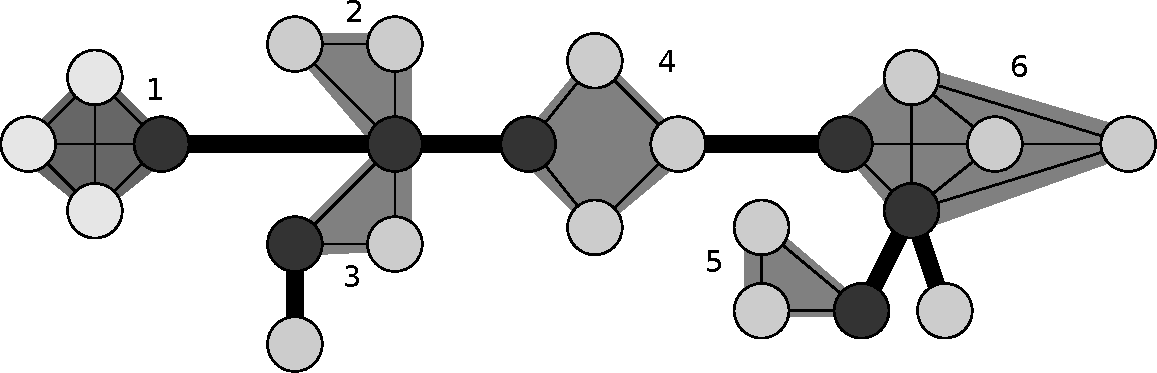
\includegraphics[width=300pt]{hw5-fig-22-10.pdf}
\end{center}
}

\end{document}


\end{document} 

